\section{Moto parabolico}
%-----------------------------------------------------------------------------
Un moto parabolico è il moto che compie un proiettile lanciato con una
certa velocità $\vec v_0$, sottoposto ad un campo di forze uniforme e
costante, ovvero il campo gravitazionale in prossimità della superficie
terrestre.\\
Il moto parabolico può essere scomposto in due moti disaccoppiati,
un moto rettilineo uniforme lungo l'asse $x$ ed un moto rettilineo
uniformemente accelerato lungo l'asse $y$. Questo perché non sono presenti
forze orizzontali, e l'unica forza agente sul corpo è quella gravitazionale
in direzione verticale. Dunque è presente un'accelerazione pari a:
$\vec a = -g\hat\jmath $. Per semplicità poniamo l'istante iniziale $ t_0 = 0$.

\begin{equation}
    \begin{cases}
        x_{(t)} = x_0 + v_0\cos\phi t\\
        y_{(t)} = y_0 + v_0\sin\phi t - \frac12 g t^2
    \end{cases}\seg
    \begin{cases}
        \dot x_{(t)} = v_0\cos\phi \\
        \dot y_{(t)} = v_0\sin\phi - gt
    \end{cases}
\label{eq:MP}
\end{equation}
\\
Si può anche ricavare l'equazione della traiettoria, isolando il tempo
dalla legge oraria per $x$ ed inserendolo nell'equazione per $y$.

\begin{equation}
    t = \frac{x-x_0}{v_0\cos\phi}\seg y_{(x)} =
    y_0 + \tan\phi\sx x-x_0\dx-\frac{g}{2v_0^2\cos^2\phi}\sx x-x_0\dx^2
\label{eq:MP_y(x)}
\end{equation}
\\
Come si può notare è l'equazione di una parabola centrata in $x_0$ con
coefficiente del termine di secondo grado sempre negativo, stante ad
indicare che la traiettoria parabolica ha sempre la concavità rivolta
verso il basso, come è giusto che sia dato che il punto materiale dovrà
cadere a terra.
\\ Imponendo la $y$ uguale a zero, possiamo ricavare il tempo di volo.

\begin{equation}
    y_0 + v_0\sin\phi \tau - \frac12 g \tau^2 = 0 \seg
    \boxed{\tau = \frac{v_0}{g}\sin\phi + \sqrt{\frac{v_0^2}{g^2}\sin^2\phi+2\frac{y_0}g}}
\label{eq:flytime}
\end{equation}
\\
Calcolando $x_{(\tau)}$ oppure imponendo uguale a zero $y_{(x)}$, otterremo
la gittata del proiettile, ovvero la massima distanza percorsa lungo
l'asse orizzontale.

\begin{equation}
    \boxed{R = x_0 + \frac{v_0^2}{g}\sin\sx\phi\dx\cos\sx\phi\dx +
    v_0\cos\phi\sqrt{\frac{v_0^2}{g^2}\sin^2\phi+2\frac{y_0}g}}
\label{eq:range}
\end{equation}
\\
Se consideriamo il caso in cui il proiettile parte da terra,
abbiamo che $y_0 = 0$ quindi la gittata diventerà:

\begin{equation}
    R = x_0 +2\frac{v_0^2}{g}\sin\sx\phi\dx\cos\sx\phi\dx = x_0 + \frac{v_0^2}{g}\sin\sx2\phi\dx
\label{eq:range_0}
\end{equation}
\\
Il valore massimo di questa $R$ si ottiene quando il $\sin\sx2\phi\dx$ è
pari ad 1, dunque la gittata massima si otterrà per $\phi = 45^\circ$.
Dobbiamo ricordare che nel caso in cui $x_0\ne0$, $R$ rappresenta
ovviamente l'ascissa del punto in cui il proiettile cade a terra.
Quindi per calcolare la distanza effettivamente percorsa, si deve
considerare la differenza $R-x_0$.
Per quanto riguarda invece la quota massima raggiunta dal proiettile,
bisogna annullare la $\dot y_{(t)}$ per ricavare il tempo in cui si
raggiunge tale quota (velocità verticale nulla).

\begin{equation}
    t^* = \frac{v_0}{g}\sin\phi\seg\boxed{h = y_0 + \frac{v_0^2}{2g}\sin^2\phi}
\label{eq:h_max}
\end{equation}
\\
\begin{figure}[h]
        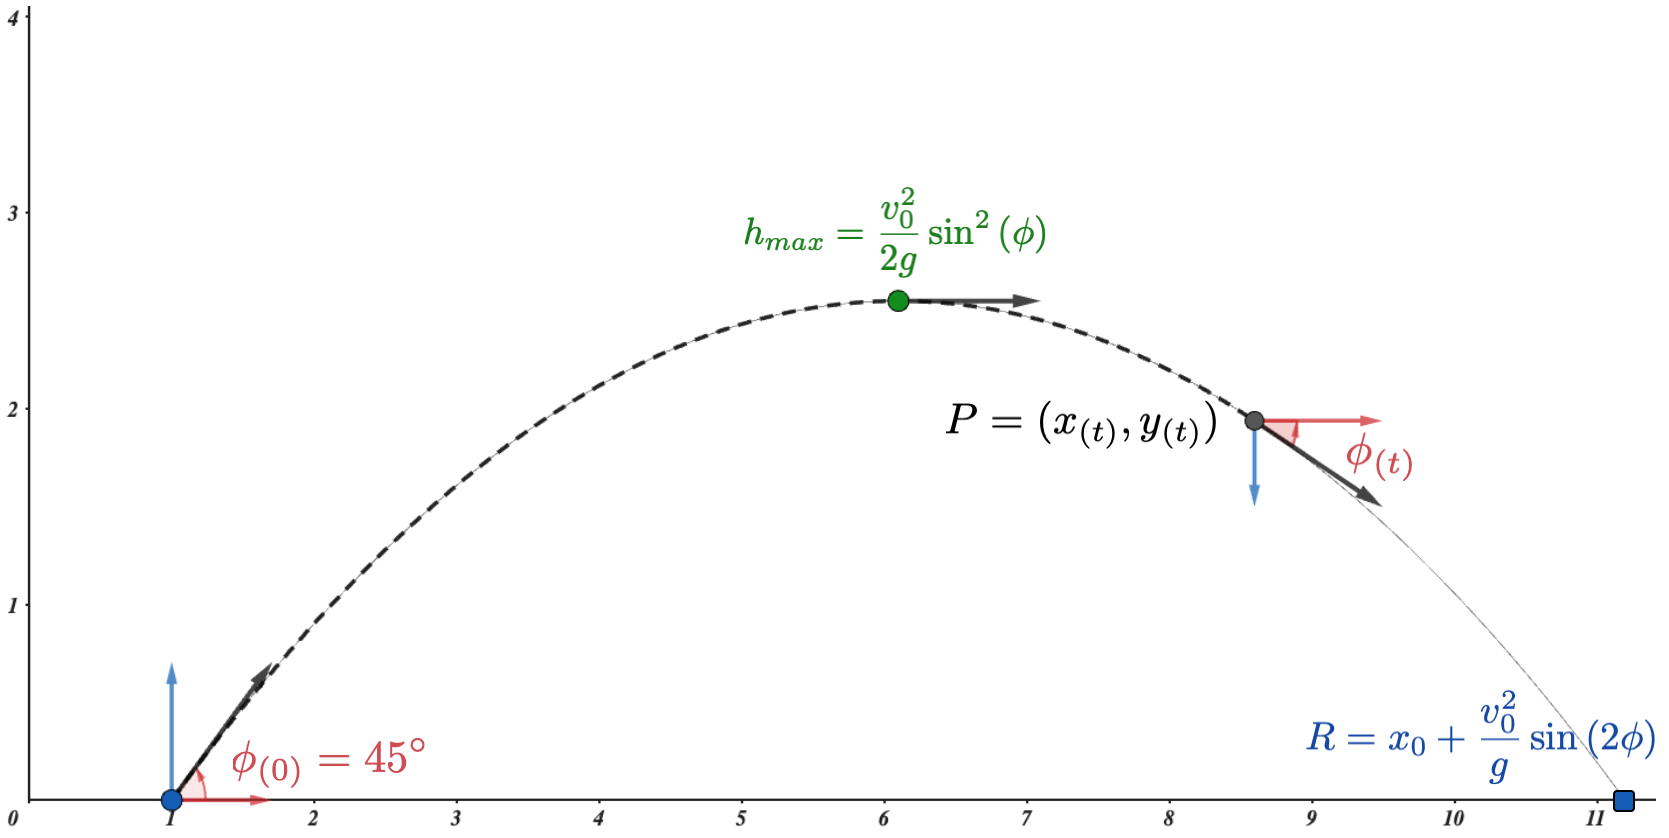
\includegraphics[width=0.9\textwidth]{images/MP1.png} 
        \caption{Esempio di una traiettoria di un moto parabolico con $\phi = 45^\circ$.
        Sono stati riportati Il punto iniziale in blu, il punto a quota
        massima in verde, un punto generico in nero ed il punto ad ascissa
        massima.}
\label{fig:MP}
\end{figure}
Se consideriamo la distanza orizzontale percorsa \emph{(gittata o range)}, oltre
al fatto di presentare un massimo $\phi = 45^\circ$, possiamo notare che si avranno
gittate uguali per angoli di lancio complementari.\\
Mostriamo qualche esempio nelle figure (\ref{fig:MP}) e (\ref{fig:MP_2}).

\begin{figure}[h]
        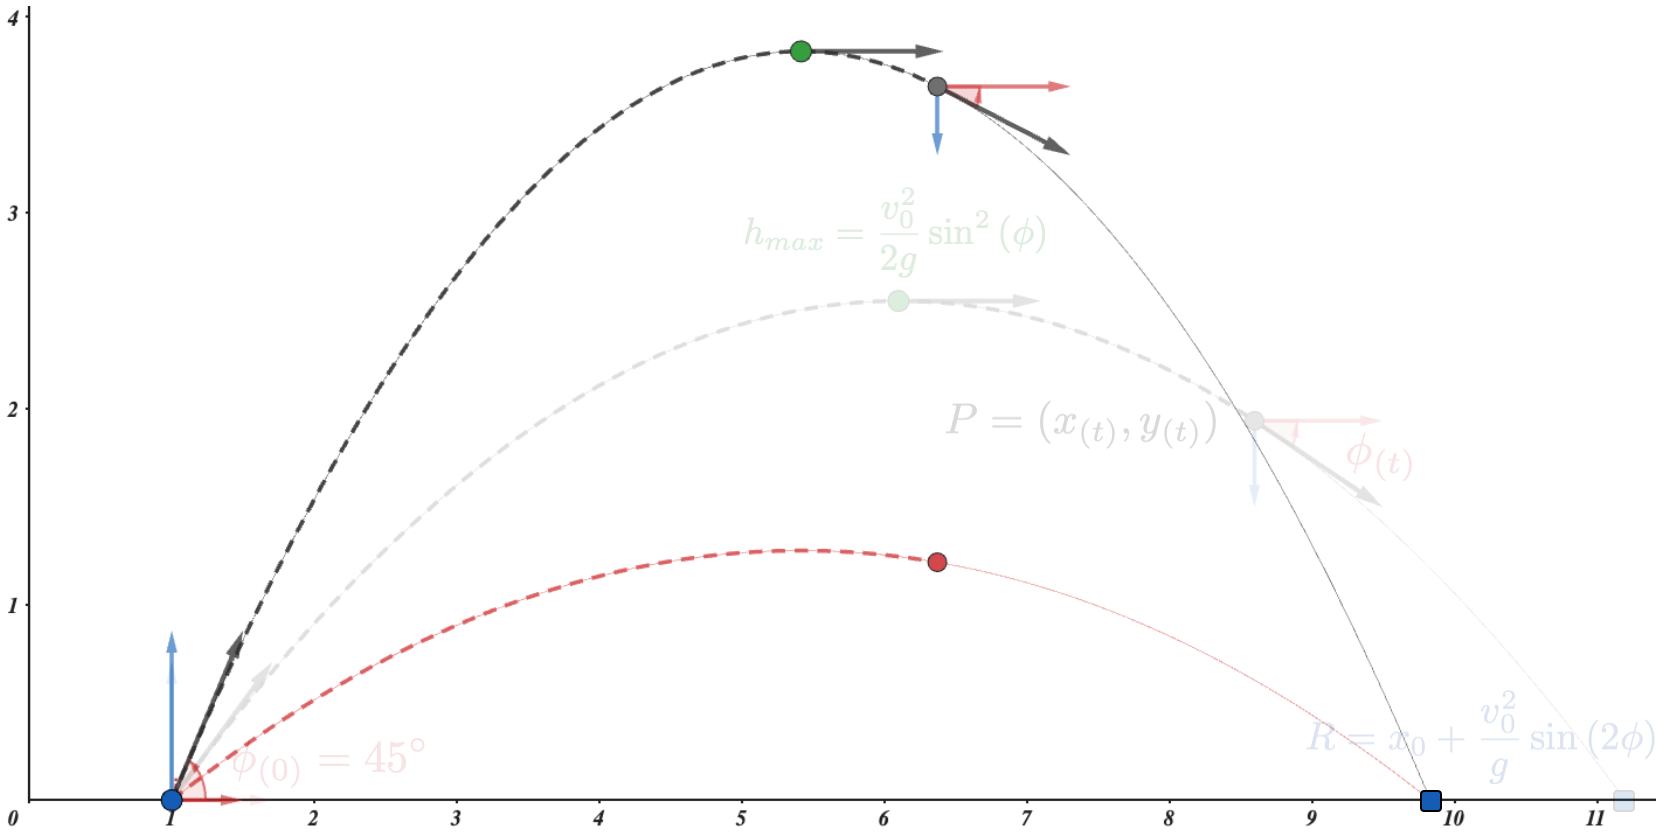
\includegraphics[width=0.9\textwidth]{images/MP2.png} 
        \caption{Rappresentazione di due traiettorie con stessa gittata.
        $\phi = 30^\circ$ in rosso e $\phi = 60^\circ$ in nero.}
\label{fig:MP_2}
\end{figure}